% %%%%%%%%%%%%%%%%%%%%%%%%%%%%%%%%%%%%%%%%%%%%%%%%%%%%%%%%%%%%%%%%%%%%%%%%%%%%%%%
\documentclass[letterpaper, 10 pt, conference]{ieeeconf}


\overrideIEEEmargins                                      % Needed to meet printer requirements.

\IEEEoverridecommandlockouts                              % This command is only needed if 
% you want to use the \thanks command

% include the list of acronyms, math commands and new commands used in this paper
% \usepackage[backend=bibtex,maxnames=2]{biblatex}
\usepackage[pdftex]{graphicx}
\usepackage[numbers]{natbib}
\bibliographystyle{IEEEtran}
\usepackage{booktabs}
\usepackage{moreverb}
%\usepackage{titlesec}
%\usepackage[titletoc,toc,title]{appendix}
\usepackage{url}
\usepackage{amsmath,amssymb}
\usepackage{multicol,lipsum}

\usepackage{bm}
\usepackage{subfig}
\usepackage{color, colortbl}
\usepackage[colorlinks,bookmarksopen,bookmarksnumbered,citecolor=red,urlcolor=red]{hyperref}


\usepackage{enumitem}

\hypersetup
{
	pdftitle = {Whole-body control for quadrupedal locomotion on challenging terrain},
	pdfauthor = {Shamel Fahmi},
	pdfsubject = {RA-L manuscript},
	pdfkeywords = {whole-body control, legged robots, challenging locomotion, and
	terrain mapping},
	pdftoolbar = true,
	colorlinks = true,
	linkcolor = black,
	citecolor = black,
	urlcolor = black,
}

\usepackage[usenames,dvipsnames]{xcolor}%\usepackage{xcolor,colortbl}
\definecolor{blue_iit}{RGB}{51,51,255}
\usepackage{algpseudocode}
\usepackage{algorithm}
\usepackage{glossaries}
\usepackage[tight]{units}
\usepackage[normalem]{ulem} % to strike out text, use: \sout{text}
\usepackage{cancel}
\definecolor{Gray}{gray}{0.9}

%\usepackage{cleveref}
%\crefname{figure}{Fig.}{Fig.}
%\crefname{equation}{Eq.}{Eq.}
%\AtBeginDocument{%
%  \renewcommand{\crefpairconjunction}{,}%% instead of " and\nobreakspace"
%  \renewcommand{\crefmiddleconjunction}{,}% instead of ", "
%  \renewcommand{\creflastconjunction}{,}% instead of " and\nobreakspace"
%}

\input{includes/acronyms.tex}
\input{includes/math_commands.tex}
\newcommand{\sref}[1]{Section~\ref{#1}}
%\newcommand{\eref}[1]{Eq.~(\ref{#1})}
\newcommand{\eref}[1]{(\ref{#1})}
\newcommand{\fref}[1]{Fig.~\ref{#1}}
\newcommand{\tref}[1]{Table~\ref{#1}}



%\newtheorem{Assumption}{Assumption}[section]
\newtheorem{assump}{Assumption}
\newtheorem{assumpB}{Assumption}
\renewcommand\theassump{1}
\renewcommand\theassumpB{2}
\newcommand{\assref}[1]{Assumption~\ref{#1}}



\newcommand{\MF}[1]{\textcolor{red}{\textbf{mfocchi}: #1}}
\newcommand{\LP}[1]{\textcolor{violet}{\textbf{lpalopoli}: #1}}
\newcommand{\ADP}[1]{\textcolor{blue}{\textbf{adelprete}: #1}}




\newcommand\BibTeX{{\rmfamily B\kern-.05em \textsc{i\kern-.025em b}\kern-.08em
T\kern-.1667em\lower.7ex\hbox{E}\kern-.125emX}}


\newcommand{\ie}{{i.e.},\ }
\newcommand{\eg}{{e.g.},\ }
\newcommand{\etal}{{\textit{et~al.}}\ }






%\usepackage[table]{xcolor}
%\definecolor{DarkGray}{RGB}{0.25,0.25,0.25}
%\definecolor{Gray}{RGB}{0.5,0.5,0.5}
%\definecolor{Red}{RGB}{1,0,0}
\definecolor{LightBlue}{RGB}{0.4,0.4,1}
\newcommand{\thickhline}{\noalign{\hrule height 0.8pt}}

\newcommand{\bmcolor}[1]{\textcolor{RoyalBlue}{\bm{#1}}}



\title{\LARGE \bf CLIO: a Novel Robotic Solution for Exploration and Rescue Missions in Hostile Mountain Environments}
\author{Michele Focchi$^{1}$, Mohamed Bensaadallah$^{2}$, Marco Frego$^{3}$, Angelika Peer$^{3}$, \\Daniele Fontanelli$^{4}$, Andrea Del Prete$^{4}$, Luigi Palopoli$^{1}$\vspace{-1.0cm}
\thanks{$^1$ The authors are with the Dipartimento di Ingegneria and Scienza dell'Informazione (DISI), University of Trento. Email:  \href{mailto:name.surname@unitn.it}{name.surname@unitn.it}}
\thanks{$^2$ The author is with the Department of Electronics, University of Batna 2, Algeria. Email: \href{mailto:m.bensaadallah@univ-batna2.dz}{m.bensaadallah@univ-batna2.dz}}
\thanks{$^3$ The authors are with the Faculty of Science and Technology, Free University of Bozen-Bolzano. Email:  \href{mailto:name.surname@unibz.it}{name.surname@unibz.it}}
\thanks{$^4$ The authors are with Dipartimento di Ingegneria Industriale (DII), University of Trento Email:  \href{mailto:name.surname@unitn.it}{name.surname@unitn.it}. The publication was created with the co-financing of the European Union FSE-REACT-EU, PON Research and Innovation 2014-2020 DM1062 / 2021.} }


\begin{document}
\maketitle
\thispagestyle{empty}
\pagestyle{empty}


\begin{abstract}%150-250 word abstract
  Rescue missions in mountain environments are hardly achievable by
  standard legged robots---because of the high slopes---or by flying
  robots---because of limited payload capacity.  We present a 
  concept for a rope-aided climbing robot which can negotiate
  up-to-vertical slopes and carry heavy payloads.  The robot is
  attached to the mountain through a rope, and it is equipped with a leg
  to push against the mountain and initiate jumping maneuvers.
  Between jumps, a hoist is used to wind/unwind the rope to move
  vertically and affect the lateral motion.  This simple (yet
  effective) two-fold actuation allows the system to achieve high
  safety and energy efficiency. Indeed, the rope prevents the robot
  from falling while compensating for most of its weight, drastically
  reducing the effort required by the leg actuator. We also present an
  optimal control strategy to generate point-to-point trajectories
  overcoming an obstacle.  We achieve fast computation time ($<$1 s)
  thanks to the use of a custom simplified robot model.  We validated
  the generated optimal movements in Gazebo simulations with a
  complete robot model with a $<5\%$ error on a 16 $m$ long jump, 
  showing the effectiveness of the proposed
  approach, and confirming the interest of our concept.  Finally, we
  performed a reachability analysis showing that the region of
  achievable targets is strongly affected by the friction properties
  of the foot-wall contact.
\end{abstract}


\section{Introduction}\label{sec:introduction}

% Strong background references addresses "what is already known" 
A climbing robot is a robot that moves on a vertical surfaces.
The idea was first suggested in a seminal work by Nishi et al.\cite{Nishi1986}
and has been revisited throughout for different application domains, 
including
%% The idea of developing climbing robots was expected for years but only in 1986, 
%% Nishi et al. presented in their seminal paper \cite{Nishi1986} 
%% the design of a robot that can walk on a vertical surface. During the last thirty years, many 
%% prototypes of climbing robots have been proposed for specific applications to replace 
%% humans in dangerous and difficult tasks, including inspection of
nuclear power 
plants \cite{Briones1994}, high-rise building cleaning \cite{Nansai2016}, bridges 
maintenance \cite{Wang2016}, search and rescue missions \cite{Eich2008}. 
However, % Mention a Gap in knowledge
there are still ways to climb walls not yet studied or reported \cite{bio_inspired2015}. 

% Introduction of the problem 
The research work done so far on climbing robots is reviewed and classified in 
\cite{Fang2022} and \cite{A.Hajeeretall2020}, respectively, according to the
adhesion technique \cite{longo2008} used to attach the robot to the
wall surface, and locomotion mechanism \cite{Chu2010}, utilized for
climbing.  The attachment and motion mechanisms are basically
considered as the main problems when designing climbing
robots. Additional requirements of equal importance come from the
application and include (R1) safety, and (R2) quickness in emergency
situations, (R3) carrying payloads, and (R4) avoiding
obstacles \cite{Schmidt2013}.

% Summarizing what's coming in the introduction
%In the coming two paragraphs, we give the reasons behind using a rope/wire 
%as an attachment method. After that, we suggest the jumping as moving technique.

\begin{figure}[t]
	\centering
	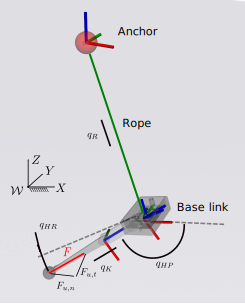
\includegraphics[width=0.7\columnwidth]{figs/3dmodel.pdf}
	\caption{\small Kinematic model of the CLIO robot with  standard definitions. The anchor frame is aligned with an inertial ($\mathcal{W}$) frame.}
	\label{fig:3dmodel}
\end{figure}


%% Solution for Attachment technique : USING A ROPE + main advantages   
Human climbers inspired the use of a rope mainly for safety measures (R1)
to support the weight of people during facade cleaning, firefighting and rescue missions
\cite{Nansai2016}.
In this paper, we combine the use of a rope with a leg, which can be retracted and extended
very quickly. This allows the robot to jump away from the mountain wall, while the rope
can be used to control its motion.

%Legged robots---as well as mobile robots---cannot walk on slopes with too high inclinations \cite{Abdalla12020} because limited friction results in slippage and falling.
%Instead, using a rope introduces an external force to compensate 
%for gravity (along the rope direction) and 
%allows the contact forces to satisfy the friction constraints (i.e., laying in 
%the middle of the friction cones) which ensures inherent safety (R1).
%
%% second advantage of using a rope : increase speed of movment 
Additionally, as shown by Wang et al. \cite{Wang2014} on dragline 
locomotion bio-inspired from spiders, the aid of rope can dramatically increase the locomotion speed (R2) 
by a winding and releasing mechanism, therefore being a preferable solution in applications
that require a prompt intervention such as Search $\&$ Rescue missions.  
%  
%% Third advantage 
Furthermore, ropes can support much heavier payloads (R3) than robots relying on sticky/adhesive approaches~\cite{Kim2008,Riskin2009}, because of the limited tangential component of the adhesive and leg actuation.
%the amount of payload that can be carried by sticky/adhesive based climbing 
%robots \cite{Kim2008,Riskin2009} is very limited due to the small tangential component of 
%the adhesive and leg actuation. Conversely, a feature of rope to be ideally 
%inextensible\footnote{The maximum payload will be limited by the maximum force deliverable 
%by the winding mechanism, e.g. a hoist, which can be extended using a gearbox.} \ADP{I don't see the connection between the rope being inextensible and the payload. The payload is large because gravity is compensated through the rope force instead of the contact force with the wall.}
%will allow the robot to carry a heavier payload (R3). 
%Difficulties due to the dynamics when using a rope
However, having the robot attached to a rope poses some challenges.
First, the robot is under-actuated because it cannot \textit{fully} control the position of its center of mass when 
not in contact with the wall. Second, the rope represents a \textit{unilateral} 
constraint (i.e. it can only pull and not push), which further complicates the already hybrid 
dynamics and the low control authority of this class of robots. 

% Providing a solution for second problem: locomotion technique, we can reach the target with jumps 
Finally, rather than slowly taking steps as walking mechanism, the robot can take one or multiple 
jumps like the rapid jumping Salto-1P shown in \cite{Haldane2017} to reach the desired locations, 
and overcoming obstacles.

%Difficulties in the jumping technique
To summarise, the key features of jumping with a rope that can be released, 
are related to the locomotion speed and the 
ability to address up to \textit{vertical} inclinations. 
However, the resulting motion of the 
robot (and so the possibility to reach the target) depends on: 1) the
impulse exerted on the wall at lift-off, 2) the winding/unwinding of the rope.
%
%Optimization for plannig 
Therefore, a planning strategy for this kind of motions should take 
into account both these factors, besides the under-actuation, 
the constraints posed by the rope, the actuator limits and the 
contact interaction (i.e. friction). 

Numerical optimisation is an attractive solution for these 
planning problems \cite{Nguyen2019,Ding2020}, since it allows to minimise some optimality criteria, 
while ensuring that the physical constraints are satisfied along the planning horizon. 
%
%Indeed, casting locomotion planning as an optimization problem
%allows one to represent high-level tasks and system dynamics using cost functions and 
%constraints. 
In this framework, different goals can also be pursued, such as minimising energy 
consumption or reaching the target in minimum time. 

\subsection{Proposed Approach and Contribution}
%
In this work, we present a novel robotic platform called CLIO  (CLImbing rObot) that is able to 
reach desired targets on a vertical (or slanted) wall with different frictional properties. 
We also propose a planning approach, based on numerical optimisation, 
to solve the jumping problem employing a simplified model of the dynamics.
To summarize, the contributions of the paper are:
\begin{itemize}
	\item a novel design of a jumping robot platform CLIO.
	\item an optimal control formulation to generate a jump 
	motion to reach a desired target while overcoming an obstacle, 
	based on a simplified model of the system, which results in reduced computation time.
	\item simulation experiments to validate the effectiveness of the proposed approach, 
	both using the simplified model and in a more realistic (Gazebo) simulation, considering the 
	full dynamics of the robot.
	\item (minor) a reachability analysis that  shows that 
	the region of achievable targets is limited by the friction coefficient at the lift-off location.
\end{itemize}
%
%\subsection{Outline}
%
The paper is organized as follows: Section \ref{sec:robot} gives an
overview of the robot platform and derives a simplified model of it.  
Section \ref{sec:motionP}  describes the optimization
problem to plan jump trajectories based on the simplified model. 
Simulations results are presented in Section \ref{sec:results}. 
Finally, we draw the conclusions in Section \ref{sec:conclusion}.


\section{Robot Description}\label{sec:robot}

\subsection{Simplified Model}
We can define a simplified mathematical model by making the following assumptions: 1. The mass is entirely concentrated in the body attached to the wire, 2. We can unwind and rewind the wire but it is rigid and remains completely elongated (i.e., it cannot make bends), 3. The rewinder can pull the wire when winding it but cannot push it (i.e., it can only act as a brake during the unwinding phase).
A geometric sketch of the system is shown in Figure \ref{fig:sp}. where the polar angle is $\theta$ [rad], the Azimuth angle $\phi$ [rad], and $l$ [m] is the length of the rigid rope. 

\begin{figure}
\includegraphics[width=\columnwidth]{figs/spherical_pendulum}
\caption{Logical scheme for the simplified model}
\label{fig:sp}
\end{figure}
Our input variables to the system are: 1. the rewinder pull action or
braking action $\mathbf{F}_r$ oriented along the wire, 2. an impulsive
push force $\mathbf{F}_u$ that the robot can generate when it is
attached to the mountain wall. 

Let $e$ be a frame attached to the mass
and with axis oriented along the $x$ axis, and let $w$ be the world
frame attached to the suspension point of the pendulum.  If we
consider the homogeneous transformation linking $e$ to $w$, we can
write:
	\[
	T_e^w = \begin{bmatrix} R_z(\phi) &\begin{matrix}0\\0\\0 \end{matrix}  \\ \begin{matrix} 0 &0 &0 \end{matrix} & 1\end{bmatrix}  \begin{bmatrix} R_y(\pi/2 - \theta) &\begin{matrix}0\\0\\0 \end{matrix}  \\ \begin{matrix} 0 &0 &0 \end{matrix} & 1\end{bmatrix}  \begin{bmatrix} I_{3,3} &\begin{matrix}0\\0\\0 \end{matrix}  \\ \begin{matrix} L &0 &0 \end{matrix} & 1\end{bmatrix}  
	\]
where $R_z(\phi)$ is the rotation matrix of $\phi$ around $z$ , and $R_y(\alpha)$ is the rotation matrix of $\alpha$ around $y$. 
Simplifying $T_e^w$, gives :
	\[
	T_e^w = \begin{bmatrix} c_\phi s_\theta & -s_\phi & c_\phi c_\theta & l c_\phi s_\theta\\
		s_\phi s_\theta & c_\phi & c_\theta s_\phi & l s_\phi s_\theta\\
		-c_\theta & 0 & s_\theta &-l c_\theta\\
		0 & 0 &0 &1\end{bmatrix} 
	\]		
where $c_x$ is a shorthand for $\cos x$ , and $s_x$ is a shorthand for $\sin x$.
The position $\mathbf{p}$ of the mass can be extracted from the transformation matrix $T_e^w$ as : 
	\begin{align}  
		\mathbf{p} = \begin{bmatrix} x\\ y\\ z \end{bmatrix} =
		\begin{bmatrix}   
            l s_\theta c_\phi\\
			l s_\theta s_\phi\\
			-l c_\theta \end{bmatrix} \label{eq1}
    \end{align}
%From equation \ref{eq1}, we can compute the velocities and the kinetic energy:   
From equation \eqref{eq1}, the velocities along Cartesian axes are    
\begin{align*}
	\dot{x} &= 
	l c_\theta c_\phi \dot{\theta} - l s_\theta s_\phi \dot{\phi} + s_\theta c_\phi \dot{l} \\
	\dot{y} &= l c_\theta s_\phi \dot{\theta} + l s_\theta c_\phi \dot{\phi} + s_\theta s_\phi \dot{l} \\
	\dot{z} &= l s_\theta  \dot{\theta} - c_\theta \dot{l} 
\end{align*}
Next, the velocity squared of the mass 
\begin{align*}
	v^2 &= \dot{x}^2 + \dot{y}^2 + \dot{z}^2 =  l^2 \dot{\theta}^2 + l^2 s_\theta^2 \dot{\phi}^2 + \dot{l}^2 		
%	&=  l^2 \dot{\theta}^2 + l^2 s_\theta^2 \dot{\phi}^2 + \dot{l}^2\\
\end{align*}
Thus, the kinetic energy $T$ and potential energy $V$  
\begin{align*}
	T &=\frac{ m }{2} v^2 =  \frac{m}{2} l^2 \left(\dot{\theta}^2 + s_\theta^2 \dot{\phi}^2 \right) + \frac{m }{2} \dot{l}^2  \\
    V &= mgz = -mgl c_\theta   \label{eq3}
\end{align*}
which leading to the Lagrangian described as
\begin{equation}
	L = T - V = \frac{m}{2} l^2 \left(\dot{\theta}^2 + s_\theta^2 \dot{\phi}^2\right) + \frac{m}{2}\dot{l}^2 + mgl c_\theta
\end{equation}
The dynamics of the system will be obtained using the Euler-Lagrange equation:
\[
\frac{d}{dt}\frac{\partial L}{\partial \dot{q}_i} - \frac{\partial L}{\partial q_i} = Q_i^p ,
\]
where $Q_i^p = (\mathbf{F}_r + \mathbf{F}_u) \cdot \frac{\partial \mathbf{p}}{\partial q_i}$ is the generalized force, 	
	$\mathbf{F}_r$ is oriented along the rope, and $\mathbf{F}_u$ is generated so that it does not have any component along the rope.
	\begin{equation}
	\begin{aligned}
		\mathbf{F}_r  &= F_r \begin{bmatrix}
			c_\phi s_\theta\\
			s_\phi s_\theta\\
			-c_\theta
		\end{bmatrix}^T = F_r \mathbf{f}_r \\	
		\mathbf{F}_u &= F_{u,t}\begin{bmatrix}
			-s_\phi\\
			c_\phi\\
			0
		\end{bmatrix}^T + F_{u,n} \begin{bmatrix}
			c_\phi c_\theta \\
			s_\phi c_\theta\\
			s_\theta
		\end{bmatrix}^T &= F_{u,t} \mathbf{f}_{u,t} + F_{u,n} \mathbf{f}_{u,n}    	 
	\end{aligned}
	\label{eq:forces}
	\end{equation}
	Let the generalized coordinates $q_i$ be chosen as $q_1 = \theta$, $q_2 = \phi$ and $q_3 = l$ . The corresponding velocities are 
	\begin{align*}
		\frac{\partial \mathbf{p}}{\partial q_1} = \frac{\partial \mathbf{p}}{\partial \theta} &= \begin{bmatrix}
			l c_\phi c_\theta\\
			l s_\phi c_\theta\\
			l s_\theta
		\end{bmatrix},  \quad \text{and} \quad 
		\frac{\partial \mathbf{p}}{\partial q_2} = \frac{\partial \mathbf{p}}{\partial \phi} &= \begin{bmatrix}
			- l s_\phi s_\theta\\
			l c_\phi s_\theta\\
			0
		\end{bmatrix}, \\
		\frac{\partial \mathbf{p}}{\partial q_3} = \frac{\partial \mathbf{p}}{\partial l} &= \begin{bmatrix}
			c_\phi s_\theta\\
			s_\phi s_\theta\\
			-c_\theta
		\end{bmatrix} .
	\end{align*}
	Hence,
\begin{align*}
	Q_1^p &= \left(\mathbf{F}_r + \mathbf{F}_u\right)   \frac{\partial \mathbf{p}}{\partial q_1} 
	%% 		&= F_r \mathbf{f}_r \cdot  \frac{\partial \mathbf{p}}{\partial \theta} + \\
	%% 		&+ F_{u,t} \mathbf{f}_{u,t} \cdot  \frac{\partial \mathbf{p}}{\partial \theta} + \\
	%% 		&+ F_{u,n} \mathbf{f}_{u,n} \cdot  \frac{\partial \mathbf{p}}{\partial \theta}  =  \\
	%% 		&= F_{u,n} \mathbf{f}_{u,n} \cdot  \frac{\partial \mathbf{p}}{\partial \theta} = \\
	= F_{u,n} l , \\
	% 	\end{align*}
% 	\begin{align*}
	Q_2^p &= \left(\mathbf{F}_r + \mathbf{F}_u\right)   \frac{\partial \mathbf{p}}{\partial q_2}
	%% 		&= F_r \mathbf{f}_r \cdot  \frac{\partial \mathbf{p}}{\partial \phi} + \\
	%% 		&+ F_{u,t} \mathbf{f}_{u,t} \cdot  \frac{\partial \mathbf{p}}{\partial \phi} + \\
	%% 		&+ F_{u,n} \mathbf{f}_{u,n} \cdot  \frac{\partial \mathbf{p}}{\partial \phi}   = \\
	%% 		&= F_{u,t} \mathbf{f}_{u,t} \cdot  \frac{\partial \mathbf{p}}{\partial \phi} =\\
	= F_{u,t} l s_\theta,\\
	%% 	\end{align*}
%% 	\begin{align*}
	Q_3^p &= \left(\mathbf{F}_r + \mathbf{F}_u\right)   \frac{\partial \mathbf{p}}{\partial q_3}
	%% 		&= F_r \mathbf{f}_r \cdot  \frac{\partial \mathbf{p}}{\partial l} + \\
	%% 		&+ F_{u,t} \mathbf{f}_{u,t} \cdot  \frac{\partial \mathbf{p}}{\partial l} + \\
	%% 		&+ F_{u,n} \mathbf{f}_{u,n} \cdot  \frac{\partial \mathbf{p}}{\partial l}   = \\
	%% 		&= F_r \mathbf{f}_r \cdot  \frac{\partial \mathbf{p}}{\partial l} =\\
	= F_{r} .
\end{align*}
With the defined generalized coordinates, The Euler-Lagrange equations gives us : 	
%% 	The first Euler-Lagrange equation yields
 	\begin{align*}
%		&\frac{d}{dt}\left(\frac{\partial L}{\partial \dot{\theta}} \right) - \frac{\partial L}{\partial \theta} = Q_1^p  \rightarrow  \\
%%		& \frac{d}{dt}\left(m l^2 \dot{\theta}\right) - (m l^2 s_\theta c_\theta \dot{\phi}^2 - m g l s_\theta) = F_{u,n}  l \\ 
 		  &m l^2 \ddot{\theta} + 2 m l \dot{\theta} \dot{l} - m l^2 s_\theta c_\theta \dot{\phi}^2 + m g l s_\theta = F_{u,n} . l\\
%% 		& \ddot{\theta} + \frac{2}{l} \dot{\theta} \dot{l} - c_\theta s_\theta \dot{\phi}^2 + \frac{g}{l}  s_\theta =  \frac{F_{u,n}  }{ml}    
%% 	\end{align*}
%% 	The second Euler-Lagrange equation yields
%% 	\begin{align*}
%% 		&\frac{d}{dt}\left(\frac{\partial L}{\partial \dot{\phi}} \right) - \frac{\partial L}{\partial \phi} = Q_2^p    \\
%% 		&\frac{d}{dt}\left(m l^2 s_\theta^2 \dot{\phi}\right) = F_{u,t}  l  s_\theta\\
 		 &\ddot{\phi} ml^2 s^2_\theta + 2 m l \dot{l} s_\theta^2 \dot{\phi} + 2 m l^2 s_\theta c_\theta \dot{\theta} \dot{\phi}  = F_{u,t}  l  s_\theta\\
%%		&\ddot{\phi} + 2 \frac{c_\theta}{s_\theta} \dot{\theta} \dot{\phi} + \frac{2}{l} \dot{\phi} \dot{l} = \frac{F_{u,t}}{ml s_\theta}
%% 	\end{align*}
%% 	The third Euler-Lagrange equation is as follows:
%% 	\begin{align*}
%% 		&\frac{d}{dt}\left(\frac{\partial L}{\partial \dot{l}} \right) - \frac{\partial L}{\partial l} = Q_3^p    \\
%% 		&\frac{d}{dt}\left(m\dot{l}\right) - (m l \dot{\theta}^2 + m l s^2_\theta \dot{\phi}^2 + m g c_\theta) = F_r ,
 		&m \ddot{l} - m l \dot{\theta}^2 - m l s^2_\theta \dot{\phi}^2 - m g c_\theta = F_r 
%% 		&\ddot{l} - l \dot{\theta}^2 - l s^2_\theta \dot{\phi}^2 - g c_\theta = \frac{F_r}{m} 
 	\end{align*}
           %%
        Overall, the non-linear dynamic equations of the system 
%        Overall, the nonlinear equations of the system are:
        \begin{equation}
        \begin{aligned}
		&\ddot{\theta} + \frac{2}{l} \dot{\theta} \dot{l} - c_\theta s_\theta  \dot{\phi}^2 + \frac{g}{l}  s_\theta =  \frac{1}{ml}F_{u,n} \\
		&\ddot{\phi} + 2 \frac{c_\theta}{s_\theta} \dot{\theta} \dot{\phi} + \frac{2}{l} \dot{\phi} \dot{l} = \frac{1}{ml s_\theta} F_{u,t} \\
		&\ddot{l} - l \dot{\theta}^2 - l s^2_\theta \dot{\phi}^2 - g c_\theta = \frac{1}{m} F_r .
	\end{aligned}
        \label{eq:nonlinearDyn}
        \end{equation}
        Clearly, in this derivation of the model, we have heavily
        relied on the point-mass nature of the body.  A possible issue
        could be the rotational dynamics of the body around its axis,
        which could waste energy generating unnecessary motions and
        impede the landing phase. This issue will be part of our
        future work. However, as discussed next, under reasonable
        assumptions (e.g., thrusting force oriented in the direction
        of the center of mass), the results based on the simplified
        model can be applied to a realistic system with a good approximation.

\subsection{Robot motion: problems and solution overview}
The problem of moving CLIO between two given configurations is not an
easy task.  First of all, even the simplified dynamics in
Equation~\eqref{eq:nonlinearDyn} is highly nonlinear.  Second, 
the configurations the robot moves between can be in general two 
distant points of the workspace. Therefore, it is not possible to
use the linearized dynamics.  Third, one of our
actuators, the thrusting force $\mathbf{F}_u$, has an impulsive nature
and operates at discrete time instants. Therefore, it is not possible
to use this part of the actuation in any feedback control scheme.
Finally, the way the tangential component $F_{u,t}$ is generated is by
using friction. Therefore, the two components $F_{u,n}$ and $F_{u,t}$ are linked
by a nonlinear constraints expressing the friction cone. Because the friction cone
depends on the specific point or area where the robot is pointing its leg,
this mechanism is not totally reliable (i.e., there can be significant deviation
between the generated and the exacted values of $F_{u,t}$).

In view of this complexity, we propose an approach based on two steps:
1. first a motion strategy is planned prior to starting the motion,
2. after the take of phase a motion controller operates on
$\mathbf{F}_r$ in a feedback control scheme to fix small deviation and
to secure that the robot lands close enough to the expected position.




\section{Motion Planning}\label{sec:motionP}
The motion plan for the robot is decided solving an optimal control problem \emph{a la} Pondryagin.
Generally speaking, we can set up the problem in the following way:
\begin{equation}
  \begin{aligned}
    &\text{min}_{\vect{u}(t)} l\left(\vect{x}(t),\vect{u}(t)\right)\\
    &\text{subject to}\\
    &\,\,\dot{\vect{x}} = f(\vect{x},\vect{u})\\
    &\,\,\vect{u} \in \mathcal{U}\\
    &\,\,\vect{x} \in \mathcal{X}\\
    &\,\,\vect{x}(t_0) = \vect{X}_0, \vect{x}(t_f)=\vect{X}_f.
  \end{aligned}
\end{equation}
where $\vect{x}$ is vector of state variables, $\vect{u}$ is the control input, $f(\cdot,\cdot)$ is the dynamic equation of the system,
$\mathcal{U}$ is set of admissible input values, $\mathcal{X}$ is the set of admissible states, $t_0$ and $t_f$ are the initial and final
instants ($t_f$ can also be an optimization variable) and $\vect{X}_0$ and $\vect{Y}_f$ are the desired initial and final states.
The state $\vect{x}$ in our problem is composed by 
$\vect{x}^T = \left[\theta,\,\phi,\,l,\,\dot{\theta},\,\dot{\phi},\, \dot{l}\right]^T$, while the command variables are
given by $\vect{u}^T = \left[\vect{F}_u,\,\vect{F}_t\right]^T$. The dynamic equation is derived from~\eqref{eq:nonlinearDyn}:
\begin{equation}
  \begin{aligned}
      \begin{bmatrix}
        \dot{x_1}\\\dot{x_2} \\ \dot{x_3}\\ \dot{x_4}\\ \dot{x_5}\\ \dot{x_6}\end{bmatrix}
     =
    \begin{bmatrix}
      x_4\\
       x_5\\ x_6 \\  - \frac{2}{x_3} x_4 x_6 + c_{x_1} s_{x_1}  x_5^2 - \frac{g}{x_3}  s_{x_1} +  \frac{1}{mx_3}F_{u,n}\\
       - 2 \frac{c_{x_1}}{s_{x_1}} x_4 x_5 - \frac{2}{x_3} x_5 x_6 + \frac{1}{mx_3 s_{x_1}} F_{u,t}\\
       x_3 x_4^2 + x_3 s^2_{x_1}x_5^2+g c_{x_1} +\frac{1}{m}F_r .
     \end{bmatrix}
    \end{aligned}
\end{equation}

\noindent
{\bf Terminal Constraints.}
The terminal constraints are usually expressed in the Cartesian space $[X,\,Y,\,Z,\,\dot{X},\dot{Y},\dot{Z}]^T$, and they can be expressed as a function of
the state variables inverting~\eqref{eq1} and~\eqref{eq:vel}. For instance, when time equals zero (initial conditions), we have:
\begin{equation}
  \begin{aligned}
    &x_1(t_0)= \atandue\left(-Z_0,\sqrt{X_0^2+Y_0^2}\right), \\ 
    &x_2(t_0) = \atandue(Y_0,X_0),\\
    &x_3(t_0) = \sqrt{X_0^2+Y_0^2+Z_0^2},\quad \\
    &x_4(t_0) = \frac{1}{\Lambda}\left(c_{x_{1}(t_0)} c_{x_2(t_0)} \dot{X}_0 +c_{x_1(t_0)}s_{x_2(t_0)} \dot{Y}_0+s_{x_1(t_0)}\dot{Z}_0\right)\\
    &x_5(t_0) = \frac{1}{\Lambda s_{x_1(t_0)}}\left(-s_{x_2(t_0)} \dot{X}_0) \right) + \\
    &\quad  +  \frac{1}{\Lambda s_{x_1(t_0)}} \left(c_{x_2(t_0)} - c_{x_2(t_0)} c^2_{x_1(t_0)} + c^2_{x_1(t_0)} s_{x_2(t_0)}  \right) \dot{Y}_0 \\
    &\quad + \frac{1}{2 \Lambda}\left(-c_{x_1(t_0)}\left(\sqrt{2}\sin\left(2 x_2(t_0)+\pi/4\right)-1 \right) \right) \dot{Z}_0 \\
    &x_6(t_0) = \frac{x_3(0)}{\Lambda}\left(s_{x_{1}(t_0)} c_{x_2(t_0)} \dot{X}_0 + s_{x_1(t_0)}s_{x_2(t_0)} \dot{Y}_0\right)\\
    & \quad + \frac{1}{2 \Lambda} c_{x_1(t_0)}\left(\sqrt{2} \cos\left(2 x_2(t_0)+\pi/4\right)-\frac{1}{2}\right) \dot{Z}_0 \\
    &\Lambda = x_3(t_0) \left(c_{x_2(t_0)} s_{x_2(t_0)} c^2_{x_1(t_0)} - c^2_{x_2(t_0)} c^2_{x_1(t_0)} + 1\right).
  \end{aligned}
\end{equation}

\noindent
{\bf State Constraints.}
State constraints are related to regions of the operation space that are not accessible. For instance, an irregular form of the walls
could generate obstacles that the robot 
has to overcome in order to reach its final destination. Generally speaking, the inaccessible area is modeled as
a a region whose boundary is a  surface defined in the Cartesian space. We assume that this surface can be expressed by
a differential 2D manifold expressed by $f(X,\,Y,\,Z) = 0$. Therefore the admissible region is generally given by
$f(X,\,Y,\,Z) \geq 0$ and could be non-convex. By using Equation~\eqref{eq1} we can express the Cartesian constraint
in terms of the state variables; therefore the constraint $\vect{x} \in \mathcal{X}$ can be expressed as $f_1(\vect{x}) \geq 0$, where $f_1$ is
assumed to be a $\mathcal{C}_\infty$ function.

\noindent
{\bf Actuation Constraints.}
The system actuators are given by the two forces $\mathbf{F}_r$ and $\mathbf{F}_u$.
The $\mathbf{F}_r$ force acts along the direction of the rope $\vect{f}_r$ (see Equation~\eqref{eq:forces}). Since the rope cannot push the robot 
(assumption 3, the rewinder can only pull the wire), $F_r$ can only be used to retract the robot or to slow down its descent. What is more, the force has an upper bound $F_r^{\text{max}}$ due to the actuators constraints. Therefore, the
constraints on $F_r$ can be expressed as :
\[
  0 \geq F_r \geq -F_r^{\text{max}} \quad .
\]
As regards $\mathbf{F}_u$, since it acts in a very small time reaching high peaks, we model it through a Dirac impulse: $\mathbf{F}_u   (t) = \mathbf{F}_u \delta(t)$, where
$\mathbf{F}_u$ is a vector with the two components $F_{u,t}$ and $F_{u,n}$.
The Dirac delta is by its very nature a discontinuous function and cannot be handled by the optimal control frameworks. Therefore, a smooth approximations is needed.
After different tests, our choice fell on a Gaussian function $\delta(t-t_0) \approx \frac{1}{\sqrt{2 \pi} \sigma} e^{-\frac{(t-t_0)^2}{2 \sigma^2}}$. The duration of the impulse
  is roughly given by $3 \sigma$. Given the nature of our actuation mechanism, a realistic choice is to have a duration in the order of tens of milliseconds, which obviously
  determines a remarkable height for the impulse. The maximum norm of $\mathbf{F}_n$ is obviously upper-bounded by the actuation limits:
  \[
    \sqrt{F_{u,n}^2 + F_{u,t}^2} \leq F_{u}^{\text{max}} \quad .
  \]
  Additionally, the tangential component $F_{u,t}$ is generated by the friction with the mountain wall. Hence, $F_{u,n}$ and $F_{u,t}$ are constrained by the following relation (friction cone):
\begin{align*}
F_{u,t}\leq \mu F_{u,n}
\end{align*} 
where $\mu$ is a constant depending on the nature of the terrain. For our simulation scenarios below, we have chosen $\mu = 0.8$ and $F_n^{\text{max}}=200$N.

\noindent
{\bf Cost Function.}
The cost function $l(\cdot)$ is composed of two terms: an integral component accounting for the cost accumulated during a period of time, and a terminal component, which accounts for the cost related to the final configuration fo the system.
For our system, we are interested in minimizing the interval of time $t_f - t_0$ needed to complete the mission and the kinetic energy $T(t_f)$ at the final instant. The reason for $T(t_f)$ is because when the robot lands,
it has to stop its motion and dissipate the energy through a damper (at the moment we are not considering to reuse the accumulated energy to re-bounce after landing).
Therefore, we have:
\begin{align*}
& l\left(\vect{x}(t),\vect{u}(t)\right)  = \lambda_1 \int_{t_0}^{t_f}dt + T(t_f)  \\
                                        &= \lambda_1 (t_f - t_0) + \frac{m}{2} x_3(t_f)^2 \left(x_4(t_f)^2 + s^2_{x_1(t_f)}+ x_5(t_f)^2 \right) \\
                                         &\quad+ \frac{m }{2} x_6(t_f)^2 \quad.
\end{align*}
We should observe that, in case of a difficult convergence, it is possible to "soften" some of the constraints. For instance, for the terminal constraint, it is possible to introduce a
slack variable $\Delta$ and have a constraint $\left\|\vect{x}(t_f) - \vect{X}_f\right\|^2 \leq \Delta$, where the slack $\Delta$ can be either a maximum tolerance set by the user or became part of the cost function.


%%% Local Variables:
%%% mode: latex
%%% TeX-master: "../icra22climb"
%%% End:



%\section{Motion Control} \label{sec:motionC}
%As anticipated in the system description above, one of the most
complex aspects of this system is that part of the control, the
$\vect{F}_u$ force, has an impulsive nature.  Its effect can be
modeled as an instantaneous reset of the velocities $\dot{\theta}$ and
$\dot{\phi}$, i.e., $x_4$ and $x_5$, respectively.  More precisely,
this effect is modelled using known state-of-the-art
results~\cite{dim17}, i.e.
\begin{equation}
  \label{eq:Reset}
  \begin{aligned}
    &x_4(t_0^+) = x_4(t_0^-) + \frac{1}{m x_3(t_0^-)} F_{u,n},\\
    &x_5(t_0^+) = x_5(t_0^-) +  \frac{1}{m x_3(0) \sin x_1(0)} F_{u,t} .
  \end{aligned}
\end{equation}
Due to the imprecisions in the actuators and to the lack of knowledge
on the terrain characteristics, the velocities after the reset could
differ from the expected values hence perturbing the whole trajectory.
The only possibility for fixing the deviation is to rely on the only
control variable available during the flight, i.e., the traction force
$F_r$, and use it within a feedback control law.  In this
section, we first address the controllability problem, i.e., if
such a feedback law can be found for an under-actuated system like ours. 
Second, we show how to design such a feedback control law.

\noindent
{\bf Local Reachability. } \ADP{Why don't you like subsubsections?}

Let us consider the system canonical form~\eqref{eq:NonLinStateSpace},
with the availability of the input $F_r$, while
$F_{u,n} = F_{u,t} = 0$ by means of~\eqref{eq:Reset}. \ADP{Not clear what \eqref{eq:Reset} has to do with the assumption that $F_u=0$} 
By recalling the
results in~\cite{isidori1985nonlinear}, we can compute the involutive
distribution $\Delta_n(\vect{x})$ and conclude for local reachability
iff $\Delta_n(\vect{x})$ is nonsingular. As such, consider the system
state $\vect{x}$ and the dynamic in~\eqref{eq:NonLinStateSpace},
rewritten as
\begin{equation}
  \label{eq:VecFields}
  \dot {\vect{x}} = f(\vect{x}) + g_r(\vect{x}) F_{r} ,
\end{equation}
hence the initial distribution is given by the column
\[
  \Delta_0(\vect{x}) = \{g_r(\vect{x})\} .
\]
It is then possible to derive
\[
  \Delta_1(\vect{x}) = \{\Delta_0(\vect{x}),
  [f(\vect{x}),g_r(\vect{x})]\} = \{\Delta_0(\vect{x}), [f(\vect{x}),
  \Delta_0(\vect{x})]\} ,
\]
where $[\cdot,\cdot]$ are the usual Lie bracket
operators~\cite{isidori1985nonlinear}, i.e.
\[
  [f(\vect{x}),g_r(\vect{x})] = \frac{\partial g_r(\vect{x})}{\partial
    \vect{x}}f(\vect{x}) - \frac{\partial f(\vect{x})}{\partial
    \vect{x}}g_r(\vect{x}) .
\]
It is then possible to derive in a recursive manner
\[
  \Delta_{n+1}(\vect{x}) = \{\Delta_n(\vect{x}),
  [f(\vect{x}),\Delta_n(\vect{x})]\} ,
\]
where, with a slight abuse of notation,
$[f(\vect{x}),\Delta_n(\vect{x})]$ is intended as the Lie brackets of
$f(\vect{x})$ with respect to all the vector fields of
$\Delta_n(\vect{x})$. After carrying out all the computations, it turns out that
$\dim\{\mbox{span}\{\Delta_5\}\} = 6$, i.e., the distribution is
nonsingular and, hence, the system is locally reachable.

\noindent {\bf Lyapunov-based control design. }

One possible path to design a state-feedback, Lyapunov-based
controller for the system~\eqref{eq:NonLinStateSpace} is to use the
backstepping technique~\cite{krstic1995nonlinear}. Let us define the
following Lyapunov function candidate on the subsystem of interest
\[
  V_1(x_1, x_2, x_3) = \frac{1}{2} [(x_1 - \overline x_1)^2 +
  (x_2 - \overline x_2)^2 + (x_3 - \overline x_3)^2] ,
\]
where the quantities $\overline \cdot$ are the desired, final values
and whose time derivative is simply given by
\[
  \dot V_1(x_1, x_2, l) = (x_1 - \overline x_1) \omega +
  (x_2 - \overline x_2) \psi + (l - \overline x_3) r . 
\]
\ADP{Why did you replace $x_3$ with $l$ in this equation? It seems inconsistent with the previous one.}
Hence, assuming the proportional control laws (with
$k_{x_1}, k_{x_2}, k_{x_3} > 0$)
\begin{equation}
  \label{eq:LyapBack}
  \begin{aligned}
    \omega & = - k_{x_1}  (x_1 - \overline x_1) , \\
    \psi & = - k_{x_2}  (x_2 - \overline x_2) , \\
    r & = - k_{x_3}  (l - \overline x_3) , 
  \end{aligned}
\end{equation}
we have immediately that
$[\overline x_1, \overline x_2, \overline x_3]^T$ is an asymptotically
stable equilibrium point for the subsystem. When the entire state $x$
is considered, it is possible to consider the quantities
in~\eqref{eq:LyapBack} as desired quantities and define the following
Lyapunov function candidate
\[
  V(x) = V_1(x_1, x_2, l) + \frac{1}{2} [(\omega -
  \overline\omega)^2 + (\psi + \overline\psi)^2 + (r + \overline r)^2] .
\]
The time derivative becomes
\[
  \begin{aligned}
    \dot V(x) = & \dot V_1(x_1, x_2, l) + (\omega -
    \overline\omega)
    (f_4(x) + \frac{F_{u,n}}{ml} - \dot{\overline\omega}) + \\
    & + (\psi - \overline\psi) (f_5(x) + \frac{F_{u,t}}{ml s_{x_1}} -
    \dot{\overline\psi}) + \\
    & + (r - \overline r) (f_6(x) + \frac{F_{r}}{m} - \dot{\overline
      r}) ,
  \end{aligned}
\]
where $f_i(x)$ is the $i$-th vector of the vector field $f(x)$
in~\eqref{eq:VecFields} and where we have from~\eqref{eq:LyapBack}
\[
  \begin{aligned}
    \dot{\overline\omega} & = - k_{x_1}  \omega , \\
    \dot{\overline\psi} & = - k_{x_2} \psi , \\
    \dot{\overline r} & = - k_{x_3} r . 
  \end{aligned}
\]
It is therefore immediate to notice that the Lyapunov candidate time
derivative $\dot V(x)$ is negative definite with the following control
laws (with $k_\omega, k_\psi, k_r > 0$)
\[
  \begin{aligned}
    F_{u,n} & = -ml (f_4(x) + k_\omega (\omega - \overline\omega) + k_{x_1}  \omega) , \\
    F_{u,t} & = -ml s_{x_1} (f_5(x) + k_\psi (\psi - \overline\psi) + k_\psi  \psi) , \\
    F_{r} & = -m (f_6(x) + k_r (r - \overline r) + k_{x_3} r) , \\
  \end{aligned}
\]
thus proving the asymptotic stability of the equilibrium
$[\overline x_1, \overline x_2, \overline x_3, 0, 0, 0]^T$ for the
system~\eqref{eq:CanonicalForm}.

In a more realistic case, we can assume that $F_{u,n} = F_{u,t} = 0$
right after the application of the impulsive inputs, thus we will
study how a stabilising Lyapunov-based control law can be designed
using only the input $F_r$. To this end, we first prove that the
system remains locally reachable. To this end, we define the reduced
version of~\eqref{eq:VecFields} as
\[
  \dot x = f(x) + g_r(x) F_{r} ,
\]
where the effect of the impulsive forces is supposed to be stored in
the state $x$ right after their applications. Hence, the initial
distribution is
\[
  \Delta_0 = \{g_r\} .
\]
It is then possible to derive in a recursive way
\[
  \Delta_{n+1} = \{\Delta_n, [f,\Delta_n]\} .
\]
It turns then out that $\mbox{span}\Delta_5 = 6$, i.e., the
distribution is nonsingular and, hence, the system is locally
reachable.

In this case, we assume that a reference trajectory for the angles
$x_1$ and $x_2$ is given, for example given by the first two
of~\eqref{eq:LyapBack}, for which both the first and second derivative
can be computed. We can then consider the following Lyapunov candidate
\[
  V(x) = \frac{1}{2} [(x_1 - \overline x_1)^2 + (x_2 -
  \overline x_2)^2 + (l - \overline x_3)^2 + (\omega -
  \overline\omega)^2 + (\psi + \overline\psi)^2 + r^2] ,
\]
whose time derivative is given by
\[
  \dot V(x) = (x_1 - \overline x_1) \omega + (x_2 -
  \overline x_2) \psi + (l - \overline x_3) r + h_1(\omega) + h_2(\psi)
  + r (f_6(x) + \frac{F_{r}}{m}),
\]
where
\[
  \begin{aligned}
    h_1(\omega) = & (\omega - \overline\omega) (f_4(x) -
    \dot{\overline\omega}) , \\
    h_2(\psi) = & (\psi - \overline\psi) (f_5(x) -
    \dot{\overline\psi}) . \\    
  \end{aligned}
\]
We can then build a Lyapunov control law that locally controls the
system dynamics.


%%% Local Variables:
%%% mode: latex
%%% TeX-master: "../icra22climb"
%%% End:



\section{Simulation Results}\label{sec:results}
This section presents simulation results that show that the planned impulses and the pattern of retraction force, 
result in of the optimization in Section \ref{sec:motionP} bring the robot to a desired target. 
In Fig. \ref{fig:validation} we validate  the results of the optimization comparing the trajectories for the \gls{com} 
in the case of the  simplified model (Matlab) and of the full 3D model (Gazebo) for a jump to a target at $p_f = \mat{4 & 5 &-8}$ $[m]$.
The discrepancy in the target position is mainly due to drift in the integration in the case of Matlab and to approximations in the model in case if Gazebo. 
However in both cases the norm of the error is always below XX which shows the simplified model is a good approximation for the real system.
The friction constraints are also fulfilled therefore initially the robot has to lift-off 
with an angle limited by the friction cone. However, since the target location is out of the cone (with vertex at the initial position)
the optimizer should "steer" the trajectory and therefore it dictates  an initial retraction of the rope to vary the time constant of the system, next it passivelt realeases the rope
under the action of gravity.

Additionally, we ran the optimization for  several targets on the wall (see Fig. \ref{fig:targets}) and we 
validated the output of the optimization both  with the simplified and the detailed model. 
Each optimoization provided the initial impulses ($Fun$, $Fut$), the pattern of the winding force $F_r$ and the jump duration $T_f$.
We terminate each simulation after the jump time $T_f$ is elapsed and computed the norm of the error from the target. 
The results are the reported in Table \ref{tab:sim_different_targets}. Note that, as expected, the error increases with the distance of the target.

\begin{figure}
	\includegraphics[width=\columnwidth]{figs/targets.png}
	\caption{Simulation. The red line is  the trajectory of the \gls{com} computed by the optimization, 
		the blue and black line is the simulated trajectory with Matlab and Gazebo, respectively.}
	\label{fig:targets}
\end{figure}



\begin{table}[h!]
	\caption{ Matlab simulations results}
	%	\renewcommand{\arraystretch}{1.1}
	\begin{center}
		\begin{tabular}{@{} l l l l l l @{}} \hline\hline
			\textbf{Test $\#$} \quad & \textbf{Target}           & \textbf{$T_f$} &  \textbf{$F_{un}$} & \textbf{$F_{ut}$} & \textbf{$\Vert e \Vert$ }\\ 
					    1    		 & \mat{4.0  & 5.0 &  -8} &      1.       &                      &                 &                 \\
					    2    		 & \mat{4.0  & 5.0 &  -8} &      1.       &                      &                 &                 \\
					    3    		 & \mat{4.0  & 5.0 &  -8} &      1.       &                      &                 &                 \\
					    4    		 & \mat{4.0  & 5.0 &  -8} &      1.       &                      &                 &                 \\
					    5    		 & \mat{4.0  & 5.0 &  -8} &      1.       &                      &                 &                 \\
					     6    		 & \mat{4.0  & 5.0 &  -8} &      1.       &                      &                 &                 \\
			\hline\hline 					    					    					    
		\end{tabular}
		\label{tab:sim_different_targets}
	\end{center}
\end{table}


\begin{figure}
	\includegraphics[width=\columnwidth]{matlab/sim_results.pdf}
	\caption{Simulation. Validation of the optimization results. The red line is the  trajectory of the \gls{com} computed by the optimization. 
		The blue and black lines are the simulated trajectory with Matlab and Gazebo, respectively.}
	\label{fig:validation}
\end{figure}





\section{Conclusions}
\label{sec:conclusion}
We presented a  robotic solution for exploration and rescue 
missions in mountain environments such as canyons, lunar craters, etc. 
It could be employed in civil applications in scaling maintenance activity, e.g., to detach from the
mountain walls dangerous boulders,  needed to mitigate the hydro-geological risk.
%or loose and potentially unstable vegetation (a.k.a. scaling) or to apply landslide protection networks
%maintenance costs in scaling application
This would create additional market opportunities for a possible business.
Our platform combines the use of a rope of adjustable length with a jumping mechanism.
We validated the result of the optimization carried out using a simplified model 
with a fully-detailed model  simulation in Gazebo,
obtaining  $5\%$ discrepancy on a 16 $m$ jump.
% limitations
The main limitations of the actual work are the limited \textit{reachability} with 
the single anchor arrangement and the lack of descriptiveness (in terms of angular dynamics) of the simplified model.
This prevents to devise planning strategies that optimize also the orientation of the robot at the landing. 
To address the first issue, we plan to investigate a solution with two ropes with more than one anchor point to increase the reachable region on the wall;
while, for the second issue, we plan to release the point-mass approximation and considering the robot as a rigid body with
non-trivial mass geometry. In this case, the thrust action has to be combined with a way to control the rotation of the body 
and in order to ensure the proper alignment of the leg  to guarantee a safe landing.  
Last, we are working on the design of a landing controller to dissipate the excess of kinetic energy at landing, 
avoiding rebounces. All these steps are preparatory to the development of a working prototype.
%
Many important future directions have been opened by this research.
Whilst avoiding obstacles is a well-known problem for motion planning in horizontal terrain, 
the jump motion pattern determined by the ropes makes the motion-planning
problem non-standard, calling for new approaches.
Much work has to be done also in the area of motion control in order to
ensure that the planned trajectory is closely tracked during the flight. 


\small
\bibliographystyle{IEEEtran}
\bibliography{references/references}

%\section{Acknowledgements}
%The publication was created with the co-financing of the European Union FSE-REACT-EU, PON Research and Innovation 2014-2020 DM1062 / 2021.

\end{document}

